\documentclass[12pt,a4paper]{article}

% =========================================================
%  CSE 3205 Assignment (Single-file LaTeX) - A4 ONLY
%  Color Design + Graph + GitHub link
%  Human-like writing
%  UML Diagram FIXED to fully fit A4 (auto-scaled)
%  References REMOVED
% =========================================================

\usepackage[a4paper,margin=1in]{geometry}
\usepackage[T1]{fontenc}
\usepackage{lmodern}
\usepackage{microtype}

\usepackage{graphicx}
\usepackage{float}
\usepackage{amsmath}
\usepackage{enumitem}
\usepackage{booktabs}
\usepackage{array}
\usepackage{colortbl}

% ---------- Colors & Design ----------
\usepackage{xcolor}
\usepackage{titlesec}
\usepackage{fancyhdr}
\usepackage{tcolorbox}

% ---------- Links ----------
\usepackage[hidelinks]{hyperref}
\usepackage{xurl} % better line breaks for long URLs
\hypersetup{
  colorlinks=true,
  linkcolor=blue,
  urlcolor=blue,
  citecolor=blue
}

% ---------- Graphs / UML ----------
\usepackage{tikz}
\usetikzlibrary{positioning,arrows.meta,shapes.multipart,fit}
\usepackage{pgfplots}
\pgfplotsset{compat=1.18}

% ---------- Lists ----------
\setlist[itemize]{noitemsep, topsep=3pt}
\setlist[enumerate]{noitemsep, topsep=3pt}

% ---------- Theme Colors ----------
\definecolor{Primary}{HTML}{1F4E79}   % deep blue
\definecolor{Accent}{HTML}{2E7D32}    % green
\definecolor{Soft}{HTML}{F3F6FA}      % light gray-blue
\definecolor{TableHead}{HTML}{D9E2EF} % table header

% ---------- Section styling ----------
\titleformat{\section}
  {\Large\bfseries\color{Primary}}{\thesection}{0.8em}{}
\titleformat{\subsection}
  {\large\bfseries\color{Accent}}{\thesubsection}{0.8em}{}
\titleformat{\subsubsection}
  {\normalsize\bfseries\color{Primary}}{\thesubsubsection}{0.8em}{}

% ---------- Header/Footer ----------
\pagestyle{fancy}
\fancyhf{}
\lhead{\color{Primary}\textbf{CSE 3205: Software Engineering}}
\rhead{\color{Primary}\textbf{Assignment}}
\cfoot{\color{Primary}\thepage}
\renewcommand{\headrulewidth}{0.6pt}
\renewcommand{\headrule}{\hbox to\headwidth{\color{Primary}\leaders\hrule height \headrulewidth\hfill}}

% ---------- Boxes ----------
\newtcolorbox{infobox}[1]{
  colback=Soft,
  colframe=Primary,
  title=\textbf{#1},
  fonttitle=\color{Primary},
  arc=3mm,
  boxrule=0.8pt
}
\newtcolorbox{noteBox}{
  colback=white,
  colframe=Accent,
  arc=2mm,
  boxrule=0.7pt
}

% ---------- Table row colors ----------
\rowcolors{2}{Soft}{white}

% =========================================================
%  STUDENT INFORMATION
% =========================================================
\newcommand{\StudentName}{Arif Foysal Bin Haider}
\newcommand{\StudentRoll}{2103119}
\newcommand{\StudentSection}{B}
\newcommand{\StudentSeries}{21}
\newcommand{\TeacherName}{Md.\ Sozib Hossain}
\newcommand{\SubmissionDate}{12 February 2026}

% =========================================================
%  GitHub Link (NOTE: % must be escaped as \%)
% =========================================================
\newcommand{\GitHubLink}{https://github.com/TheObsidianEye-ARIF-FOYSAL/cse-3205/blob/main/CSE\%203205\%20Assignment/2103119_CSE_3205_Assignment.tex}

\begin{document}

% =========================================================
%  COVER PAGE
% =========================================================
\begin{titlepage}
\centering
\vspace*{0.4cm}

{\Large \textbf{Heaven's Light is Our Guide}\par}
\vspace{0.2cm}
{\Large \textbf{Rajshahi University of Engineering \& Technology (RUET)}\par}
\vspace{0.2cm}
{\large Department of Computer Science \& Engineering\par}

\vspace{1.0cm}
{\LARGE \textbf{Assignment}\par}
\vspace{0.7cm}

{\large \textbf{Software Process Models, Software Testing \& Quality Assurance, and Design Patterns \& Modern Software Tools}\par}

\vspace{0.9cm}

\begin{tabular}{>{\bfseries}l l}
Course Code & : CSE 3205\\
Course Title & : Software Engineering\\
Date of Submission & : \SubmissionDate\\
\end{tabular}

\vspace{1.0cm}

\begin{infobox}{GitHub Link (Code and Version History)}
\textbf{Link:} \url{\GitHubLink}\\
\end{infobox}

\vfill

\begin{minipage}{0.45\textwidth}
\textbf{Submitted by}\\[6pt]
Name : \StudentName\\
Roll : \StudentRoll\\
Section : \StudentSection\\
Series : \StudentSeries\\
\end{minipage}
\hfill
\begin{minipage}{0.45\textwidth}
\textbf{Submitted to}\\[6pt]
\TeacherName\\
Lecturer\\
Department of CSE, RUET\\
\end{minipage}

\vspace{0.8cm}
\end{titlepage}

\tableofcontents
\newpage

% =========================================================
%  ASSIGNMENT 1
% =========================================================
\section{Assignment 1: Software Process Models Analysis}

\subsection{Scenario Overview}
The company wants to build an Online Course Management System (OCMS). The main challenge is that
requirements will \textbf{change frequently} because the system must stay useful and competitive.
Also, regular feedback from students, instructors, and administrators is expected.

So, the process model should support:
\begin{itemize}
  \item fast delivery in small iterations,
  \item easy handling of changing requirements,
  \item continuous collaboration with stakeholders.
\end{itemize}

\subsection{1. Process Model Identification \& Analysis}

\subsubsection{Model 1: Agile (Scrum)}
Agile Scrum works in short cycles called \textbf{sprints}. In each sprint, the team selects a small set of
features, implements them, tests them, and delivers working software.

\begin{noteBox}
\textbf{Practical point:} After every sprint, we can show real progress. If the users want changes, the next sprint can handle it.
\end{noteBox}

\textbf{How Scrum fits OCMS}
\begin{itemize}
  \item First sprints deliver basics: login, course listing, user roles.
  \item Next sprints add enrollment, content upload, assignments, grading, analytics.
  \item Feedback is collected every sprint and used to improve the next plan.
\end{itemize}

\subsubsection{Model 2: Spiral Model}
The Spiral Model is also iterative, but it is \textbf{risk-focused}. Each cycle includes planning,
risk analysis, development, and evaluation.

\textbf{How Spiral fits OCMS}
\begin{itemize}
  \item Strong when there are big risks (security, scaling, third-party integration).
  \item More formal and heavier than Scrum, which can slow a mid-sized team.
\end{itemize}

\subsection{2. Comparative Engineering Analysis}

\begin{table}[H]
\centering
\caption{Agile (Scrum) vs Spiral Model for OCMS}
\begin{tabular}{p{3.4cm} p{5.8cm} p{5.8cm}}
\toprule
\rowcolor{TableHead}
\textbf{Metric} & \textbf{Agile (Scrum)} & \textbf{Spiral Model}\\
\midrule
Requirement Flexibility &
Very high: backlog reprioritization each sprint supports frequent changes easily. &
High but slower: changes handled per spiral cycle (usually longer).\\
\addlinespace
Risk Management &
Moderate: handled continuously, but usually not a formal “risk phase.” &
Very strong: explicit risk identification and mitigation each iteration.\\
\addlinespace
Customer Involvement &
Very frequent: sprint review gives continuous feedback. &
Frequent but milestone-based: feedback at the end of each spiral.\\
\addlinespace
Cost \& Overhead &
Lower overhead; lightweight documentation; faster iteration. &
Higher overhead because of risk analysis and documentation.\\
\addlinespace
Predictability &
Medium: flexible scope may shift across sprints. &
Higher: structured cycles give clearer checkpoints.\\
\bottomrule
\end{tabular}
\end{table}

\subsection*{Visual Comparison (Graph)}
\begin{figure}[H]
\centering
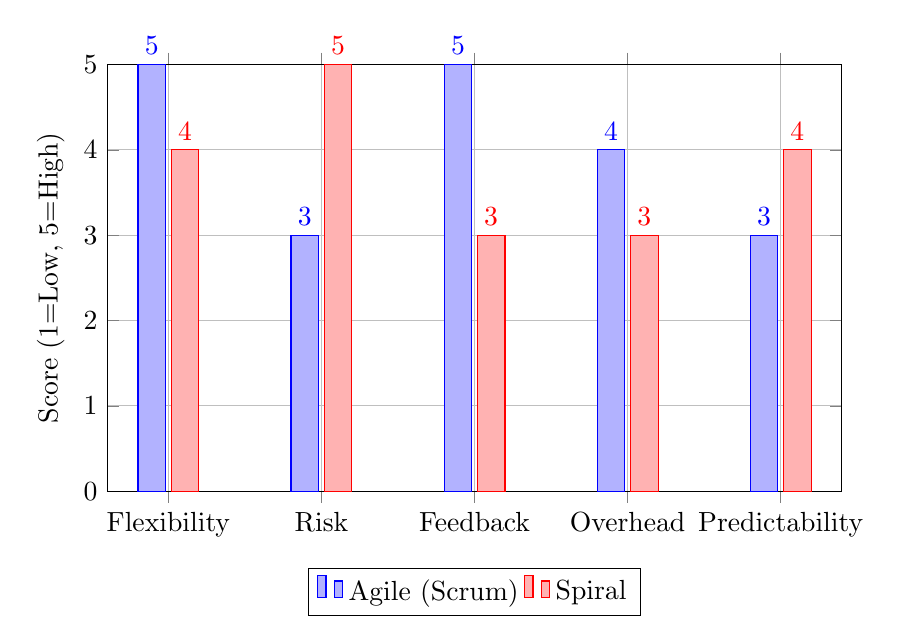
\begin{tikzpicture}
\begin{axis}[
    ybar,
    bar width=10pt,
    width=0.9\textwidth,
    height=7cm,
    ymin=0, ymax=5,
    ylabel={Score (1=Low, 5=High)},
    symbolic x coords={Flexibility,Risk,Feedback,Overhead,Predictability},
    xtick=data,
    legend style={at={(0.5,-0.18)},anchor=north,legend columns=2},
    nodes near coords,
    nodes near coords align={vertical},
    grid=both
]
\addplot coordinates {(Flexibility,5) (Risk,3) (Feedback,5) (Overhead,4) (Predictability,3)};
\addplot coordinates {(Flexibility,4) (Risk,5) (Feedback,3) (Overhead,3) (Predictability,4)};
\legend{Agile (Scrum),Spiral}
\end{axis}
\end{tikzpicture}
\caption{Agile vs Spiral (relative scoring for the OCMS case)}
\end{figure}

\subsection{3. Recommendation}
\begin{infobox}{Final Choice}
\textbf{Recommended Model: Agile (Scrum)}\\
Scrum best supports frequent requirement changes and continuous user feedback for an evolving OCMS.
\end{infobox}

In an OCMS project, priorities will change based on user needs and real usage. Scrum supports this naturally
because planning happens sprint by sprint. Spiral is excellent for high-risk projects, but for a mid-sized team
building an evolving product, Scrum is typically the more practical choice.

\newpage

% =========================================================
%  ASSIGNMENT 2
% =========================================================
\section{Assignment 2: Software Testing \& Quality Assurance Plan}

\subsection{Scenario Overview}
A Library Management System (LMS) manages book search, borrowing, returning, and user accounts.
Here, \textbf{correctness is critical}. Even small mistakes (wrong availability status, wrong fine)
create real problems in daily library operations.

\subsection{1. Testing Strategy (Four Testing Types)}
\begin{table}[H]
\centering
\caption{Testing types and what they ensure}
\begin{tabular}{p{3.2cm} p{12.0cm}}
\toprule
\rowcolor{TableHead}
\textbf{Testing Type} & \textbf{Purpose}\\
\midrule
Unit Testing & Checks individual functions (fine calculation, ISBN validation) in isolation.\\
Integration Testing & Checks interaction between modules (borrow service, DB, user account).\\
System Testing & Tests the full system end-to-end using realistic workflows.\\
Acceptance Testing (UAT) & Confirms real users can complete tasks and rules meet requirements.\\
\bottomrule
\end{tabular}
\end{table}

\subsection{2. Example Test Scenarios}

\subsubsection{Unit Test Scenario (Fine Calculation)}
\textbf{Function:} \texttt{CalculateOverdueFine(borrowDate, returnDate, periodDays)} (period=14 days, rate=\$0.50/day)
\begin{itemize}
  \item Borrow Jan 1, return Jan 21 $\Rightarrow$ overdue 6 days $\Rightarrow$ fine \$3.00
  \item Borrow Jan 1, return Jan 10 $\Rightarrow$ not overdue $\Rightarrow$ fine \$0.00
  \item Missing return date $\Rightarrow$ should throw an error / exception
\end{itemize}

\subsubsection{Integration Test Scenario (Borrow + Inventory + Account)}
\begin{itemize}
  \item Borrow available book $\Rightarrow$ record created + copies reduce by 1.
  \item Copies = 0 $\Rightarrow$ borrowing blocked with “Unavailable”.
  \item DB failure during borrow $\Rightarrow$ rollback (no partial update).
\end{itemize}

\subsubsection{System Test Scenario (Full Workflow)}
\begin{itemize}
  \item Login $\rightarrow$ Search $\rightarrow$ Borrow $\rightarrow$ Return works correctly.
  \item Availability updates immediately after return.
  \item Two users try last copy: only one succeeds.
\end{itemize}

\subsubsection{Acceptance Test Scenario (Librarian)}
\begin{itemize}
  \item Scan barcode $\rightarrow$ borrower found $\rightarrow$ fine shown $\rightarrow$ book marked Available.
  \item Fine matches manual calculation.
\end{itemize}

\subsection{3. Software Quality Assurance (SQA) Plan}

\subsubsection{Quality Goals (Measurable Targets)}
\begin{table}[H]
\centering
\caption{SQA measurable targets}
\begin{tabular}{p{4.0cm} p{6.3cm} p{4.8cm}}
\toprule
\rowcolor{TableHead}
\textbf{Quality Attribute} & \textbf{Metric} & \textbf{Target}\\
\midrule
Reliability & Uptime & 99.9\% uptime\\
Critical Defects & Sev-1 bugs in production & 0\\
Data Accuracy & Inventory mismatch rate & $\geq$ 99.99\% accurate\\
Performance & Search response time & $<2$ sec for 95\% queries\\
Test Coverage & Automated line coverage & $\geq$ 85\% (critical modules 100\%)\\
\bottomrule
\end{tabular}
\end{table}

\subsubsection{Review \& QA Activities}
\begin{itemize}
  \item \textbf{Before coding:} review requirements and confirm test cases.
  \item \textbf{During coding:} code review + static checks + unit tests in every update.
  \item \textbf{Before release:} regression + system test + UAT in staging.
  \item \textbf{After release:} monitoring logs and quick hotfix for critical issues.
\end{itemize}

\subsubsection{Defect Tracking}
\begin{infobox}{Defect Lifecycle}
New $\rightarrow$ Triaged $\rightarrow$ Assigned $\rightarrow$ In Progress $\rightarrow$ Fixed $\rightarrow$ Retest $\rightarrow$ Verified $\rightarrow$ Closed
\end{infobox}

\subsection{4. Why This Plan Works}
This approach catches issues early (unit tests), prevents broken module interactions (integration tests),
verifies real workflows (system tests), and ensures users are satisfied (UAT). Overall, it improves reliability,
keeps data correct, and reduces downtime.

\newpage

% =========================================================
%  ASSIGNMENT 3
% =========================================================
\section{Assignment 3: Design Patterns \& Modern Software Tools}

\subsection{Scenario Overview}
A Smart Home Automation System can grow over time: new devices appear, and multiple vendors provide their
own implementations. The controller should not need major code changes each time a new vendor is added.

\subsection{1. Selected Pattern}
\begin{infobox}{Selected Pattern: Abstract Factory}
Abstract Factory helps create related objects (Light, Fan, Sensor) without depending on concrete classes.
This keeps the controller clean and makes the system easier to expand later.
\end{infobox}

\subsection{2. UML Class Diagram (Abstract Factory) --- A4-Fit}
% A4-Fit trick: resize to \textwidth so it never gets cut off
\begin{figure}[H]
\centering
\resizebox{\textwidth}{!}{%
\begin{tikzpicture}[
  class/.style={
    draw=Primary, rounded corners=2mm, very thick,
    fill=Soft, text width=5.0cm, align=left, inner sep=4pt
  },
  rel/.style={-Latex, thick, draw=Primary},
  impl/.style={-Latex, thick, dashed, draw=Primary}
]

\node[class] (factory) {
\textbf{SmartDeviceFactory (interface)}\\ \hline
+ createLight(): Light\\
+ createFan(): Fan\\
+ createSensor(): Sensor
};

\node[class, below left=1.1cm and 0.5cm of factory] (philipsF) {
\textbf{PhilipsFactory}\\ \hline
+ createLight(): Light\\
+ createFan(): Fan\\
+ createSensor(): Sensor
};

\node[class, below right=1.1cm and 0.5cm of factory] (xiaomiF) {
\textbf{XiaomiFactory}\\ \hline
+ createLight(): Light\\
+ createFan(): Fan\\
+ createSensor(): Sensor
};

\draw[impl] (philipsF.north) -- (factory.south);
\draw[impl] (xiaomiF.north) -- (factory.south);

\node[class, right=1.1cm of factory, text width=4.2cm] (lightI) {
\textbf{Light (interface)}\\ \hline
+ on()\\
+ off()
};

\node[class, below=0.9cm of lightI, text width=4.2cm] (fanI) {
\textbf{Fan (interface)}\\ \hline
+ start()\\
+ stop()
};

\node[class, below=0.9cm of fanI, text width=4.2cm] (sensorI) {
\textbf{Sensor (interface)}\\ \hline
+ read(): data
};

\node[class, above=1.1cm of lightI, text width=5.0cm] (controller) {
\textbf{SmartHomeController}\\ \hline
- factory: SmartDeviceFactory\\
- devices: List\\ \hline
+ setup()\\
+ controlAll()
};

\draw[rel] (controller.west) -- (factory.east);

\draw[rel] (factory.east) to[bend left=10] (lightI.west);
\draw[rel] (factory.east) to[bend left=10] (fanI.west);
\draw[rel] (factory.east) to[bend left=10] (sensorI.west);

\end{tikzpicture}%
}
\caption{UML Class Diagram: Abstract Factory Pattern (Scaled to fit A4 width)}
\end{figure}

\subsection{3. Why This Pattern Makes Sense}
\begin{itemize}
  \item \textbf{Easy expansion:} add a new vendor factory without changing the controller.
  \item \textbf{Cleaner design:} object creation stays in factories, not scattered across the system.
  \item \textbf{Lower maintenance cost:} vendor changes are isolated, so fewer bugs appear.
\end{itemize}

\subsection{4. Modern Tool (Git) in This Context}
Git supports reliable teamwork and version control:
\begin{itemize}
  \item tracks all changes (who changed what and when),
  \item supports collaboration through branches and pull requests,
  \item helps rollback if an update causes unexpected problems.
\end{itemize}

\newpage

% =========================================================
%  CONCLUSION
% =========================================================
\section*{Conclusion}
In this assignment, I selected a process model that fits frequent changes (Scrum), designed a realistic testing and
SQA plan for correctness and reliability, and applied the Abstract Factory pattern to show how good design supports
scalability. Overall, these approaches help build software that is easier to maintain, easier to improve, and more
dependable for real users.

\end{document}
